\documentclass[10pt]{beamer}
\setbeamerfont{normal text}{size=\small}
\AtBeginDocument{\usebeamerfont{normal text}}

\usefonttheme{professionalfonts}

\usetheme[progressbar=frametitle]{metropolis}
\usepackage{appendixnumberbeamer}

\usepackage{booktabs}
\usepackage[scale=2]{ccicons}

\usepackage{pgfplots}
\usepgfplotslibrary{dateplot}

\usepackage{xspace}
\newcommand{\themename}{\textbf{\textsc{metropolis}}\xspace}

\usepackage{bm}
\usepackage[thinc]{esdiff}
\newcommand{\phdot}{{}\cdot{}}
\DeclareMathOperator{\tr}{tr}
\DeclareMathOperator{\adj}{adj}

\usepackage{xfrac}

\definecolor{plotBlue}{HTML}{00ACCE}

%%%%%%%%%%%%%%%%%%%%%%%%%%%%%%%%%%%%%%%%%%%%%%%%%%%%%%%%%%%%%%%%%%%%%%%%%%%%%%
% \embedvideo{<poster or text>}{<video file (MP4+H264)>}
% \embedvideo*{...}{...}                     % auto-play
%%%%%%%%%%%%%%%%%%%%%%%%%%%%%%%%%%%%%%%%%%%%%%%%%%%%%%%%%%%%%%%%%%%%%%%%%%%%%%
\usepackage[bigfiles]{pdfbase}
\ExplSyntaxOn
\NewDocumentCommand\embedvideo{smm}{
  \group_begin:
  \leavevmode
  \tl_if_exist:cTF{file_\file_mdfive_hash:n{#3}}{
    \tl_set_eq:Nc\video{file_\file_mdfive_hash:n{#3}}
  }{
    \IfFileExists{#3}{}{\GenericError{}{File~`#3'~not~found}{}{}}
    \pbs_pdfobj:nnn{}{fstream}{{}{#3}}
    \pbs_pdfobj:nnn{}{dict}{
      /Type/Filespec/F~(#3)/UF~(#3)
      /EF~<</F~\pbs_pdflastobj:>>
    }
    \tl_set:Nx\video{\pbs_pdflastobj:}
    \tl_gset_eq:cN{file_\file_mdfive_hash:n{#3}}\video
  }
  %
  \pbs_pdfobj:nnn{}{dict}{
    /Type/RichMediaInstance/Subtype/Video
    /Asset~\video
    /Params~<</FlashVars (
      source=#3&
      skin=SkinOverAllNoFullNoCaption.swf&
      skinAutoHide=true&
      skinBackgroundColor=0x5F5F5F&
      skinBackgroundAlpha=0.75
    )>>
  }
  %
  \pbs_pdfobj:nnn{}{dict}{
    /Type/RichMediaConfiguration/Subtype/Video
    /Instances~[\pbs_pdflastobj:]
  }
  %
  \pbs_pdfobj:nnn{}{dict}{
    /Type/RichMediaContent
    /Assets~<<
      /Names~[(#3)~\video]
    >>
    /Configurations~[\pbs_pdflastobj:]
  }
  \tl_set:Nx\rmcontent{\pbs_pdflastobj:}
  %
  \pbs_pdfobj:nnn{}{dict}{
    /Activation~<<
      /Condition/\IfBooleanTF{#1}{PV}{XA}
      /Presentation~<</Style/Embedded>>
    >>
    /Deactivation~<</Condition/PI>>
  }
  %
  \hbox_set:Nn\l_tmpa_box{#2}
  \tl_set:Nx\l_box_wd_tl{\dim_use:N\box_wd:N\l_tmpa_box}
  \tl_set:Nx\l_box_ht_tl{\dim_use:N\box_ht:N\l_tmpa_box}
  \tl_set:Nx\l_box_dp_tl{\dim_use:N\box_dp:N\l_tmpa_box}
  \pbs_pdfxform:nnnnn{1}{1}{}{}{\l_tmpa_box}
  %
  \pbs_pdfannot:nnnn{\l_box_wd_tl}{\l_box_ht_tl}{\l_box_dp_tl}{
    /Subtype/RichMedia
    /BS~<</W~0/S/S>>
    /Contents~(embedded~video~file:#3)
    /NM~(rma:#3)
    /AP~<</N~\pbs_pdflastxform:>>
    /RichMediaSettings~\pbs_pdflastobj:
    /RichMediaContent~\rmcontent
  }
  \phantom{#2}
  \group_end:
}
\ExplSyntaxOff
%%%%%%%%%%%%%%%%%%%%%%%%%%%%%%%%%%%%%%%%%%%%%%%%%%%%%%%%%%%%%%%%%%%%%%%%%%%%%%

\usepackage{biblatex}
\addbibresource{main.bib}

\AtEveryCitekey{\iffootnote{\scriptsize}{}}

\usepackage{emoji}

\title{Gatsby Bridging Program}
\subtitle{Probability: Functions of Random Variables}
% \date{\today}
\date{}
\author{Cameron Stewart}
\institute{Gatsby Computational Neuroscience Unit}
\titlegraphic{\hfill
\includegraphics[height=1.5cm]{logo.png}}

\begin{document}

\maketitle

\begin{frame}{Today's Lecture Topics}
  \setbeamertemplate{section in toc}[sections numbered]
  \tableofcontents%[hideallsubsections]
\end{frame}

\section{Prerequisites and Motivation}

\begin{frame}[fragile]{Revision: Injective, Surjective, and Bijective Functions}
Today's content will be based heavily on the concepts of injectivity, surjectivity, and bijectivity. So, here is some revision.

\(g: \mathcal{X}\rightarrow\mathcal{Y}\) implies that the function \(g\) takes elements from the set \(\mathcal{X}\) and maps them to elements of the set \(\mathcal{Y}\). \(\mathcal{X}\) is the domain and \(\mathcal{Y}\) is the codomain.\onslide<2>{

Not all elements of \(\mathcal{Y}\) may be attainable for a given function. The set of elements which are attainable is called the image, given by
\begin{equation*}
    g\left(\mathcal{X}\right) = \left\{g\left(x\right) \;\middle|\; x\in\mathcal{X}\right\}\,.
\end{equation*}
Clearly, \(g\left(\mathcal{X}\right) \subseteq \mathcal{Y}\).}
\end{frame}

\begin{frame}[fragile]{Revision: Injective Functions}
\begin{figure}
    \centering
    \begin{tikzpicture}
    \footnotesize
    \coordinate (A1) at ({cos(84.26)},{sin(84.26)});
    \coordinate (A2) at ({cos(84.26)},{-sin(84.26)});
    \coordinate (B1) at ({5+0.5*cos(84.26)}, {0.5*sin(84.26)});
    \coordinate (B2) at ({5+0.5*cos(84.26)},{-0.5*sin(84.26)});
    \draw[mLightBrown,ultra thick] (5.4,0) circle[radius=1];
    \draw[black,dotted,thick] (B2) arc[radius=0.5,start angle=-84.26,end angle=84.26] -- (A1)
      arc[radius=1,start angle=84.26,end angle=275.74] -- cycle;
    \draw[mLightGreen,ultra thick] (0,0) circle[radius=1];
    \draw[plotBlue,ultra thick] (5,0) circle[radius=.5];
    \node[align=center] at (0,0) {\(\mathcal{X}\)};
    \node[align=center] at (5,0) {\(g\left(\mathcal{X}\right)\)};
    \node[align=center] at (5.95,0) {\(\mathcal{Y}\)};
    \node[align=center] at (2.7,1.2) {\(g: \mathcal{X} \rightarrow \mathcal{Y}\)};
    \node[align=center] at (2.7,0) {One-to-one mapping\\between \(\mathcal{X}\) and \(g\left(\mathcal{X}\right)\).};
    \end{tikzpicture}
\end{figure}

\metroset{block=fill}\begin{alertblock}{Injection}
If every \(x \in \mathcal{X}\) has a unique mapped value \(g\left(x\right)\), then \(g\) is injective.
\begin{equation*}
\forall x_1, x_2 \in \mathcal{X}, g\left(x_1\right) = g\left(x_2\right) \Rightarrow x_1 = x_2
\end{equation*}
\end{alertblock}
\end{frame}

\begin{frame}[fragile]{Revision: Surjective Functions}
\begin{figure}
    \centering
    \begin{tikzpicture}
    \footnotesize
    \coordinate (A1) at ({cos(90)},{sin(90)});
    \coordinate (A2) at ({cos(90)},{-sin(90)});
    \coordinate (B1) at ({5.4+1*cos(90)}, {1*sin(90)});
    \coordinate (B2) at ({5.4+1*cos(90)},{-1*sin(90)});
    \draw[black,dotted,thick] (B2) arc[radius=1,start angle=-90,end angle=90] -- (A1)
      arc[radius=1,start angle=90,end angle=270] -- cycle;
    \draw[mLightBrown,ultra thick] (5.4,0) circle[radius=1];
    \draw[mLightGreen,ultra thick] (0,0) circle[radius=1];
    \draw[plotBlue,ultra thick, dash pattern=on 10pt off 10pt] (5.4,0) circle[radius=1];
    \node[align=center] at (0,0) {\(\mathcal{X}\)};
    \node[align=center] at (5.4,0) {\(g\left(\mathcal{X}\right) = \mathcal{Y}\)};
    \node[align=center] at (2.7,1.2) {\(g: \mathcal{X} \rightarrow \mathcal{Y}\)};
    \node[align=center] at (2.7,0) {Every element in \(\mathcal{Y}\)\\corresponds to at least\\one element in \(\mathcal{X}\).};
    \end{tikzpicture}
\end{figure}

\metroset{block=fill}\begin{alertblock}{Surjection}
If every \(y \in \mathcal{Y}\) has at least one solution to \(y = g\left(x\right)\) for \(x \in \mathcal{X}\), then \(g\) is surjective.
\begin{equation*}
\forall y \in \mathcal{Y}, \exists x \in \mathcal{X} \textrm{ such that } y = g\left(x\right)
\end{equation*}
\end{alertblock}
\end{frame}

\begin{frame}[fragile]{Revision: Bijective Functions}
\begin{figure}
    \centering
    \begin{tikzpicture}
    \footnotesize
    \coordinate (A1) at ({cos(90)},{sin(90)});
    \coordinate (A2) at ({cos(90)},{-sin(90)});
    \coordinate (B1) at ({5.4+1*cos(90)}, {1*sin(90)});
    \coordinate (B2) at ({5.4+1*cos(90)},{-1*sin(90)});
    \draw[black,dotted,thick] (B2) arc[radius=1,start angle=-90,end angle=90] -- (A1)
      arc[radius=1,start angle=90,end angle=270] -- cycle;
    \draw[mLightBrown,ultra thick] (5.4,0) circle[radius=1];
    \draw[mLightGreen,ultra thick] (0,0) circle[radius=1];
    \draw[plotBlue,ultra thick, dash pattern=on 10pt off 10pt] (5.4,0) circle[radius=1];
    \node[align=center] at (0,0) {\(\mathcal{X}\)};
    \node[align=center] at (5.4,0) {\(g\left(\mathcal{X}\right) = \mathcal{Y}\)};
    \node[align=center] at (2.7,1.2) {\(g: \mathcal{X} \rightarrow \mathcal{Y}\)};
    \node[align=center] at (2.7,0) {One-to-one mapping\\between \(\mathcal{X}\) and \(\mathcal{Y}\).};
    \end{tikzpicture}
\end{figure}

\metroset{block=fill}\begin{alertblock}{Bijection}
If \(g\) is injective and surjective, then it is called bijective.
\begin{equation*}
\forall y \in \mathcal{Y}, \href{https://en.wikipedia.org/wiki/Uniqueness_quantification}{\color{mLightBrown}{\exists!}} x \in \mathcal{X} \textrm{ such that } y = g\left(x\right)
\end{equation*}
Bijective functions have inverses. We denote \(g^{-1}\) as the inverse of \(g\).
\end{alertblock}
\end{frame}

\begin{frame}[fragile]{Revision: Injective, Surjective, and Bijective Functions}
\metroset{block=fill}\begin{exampleblock}{Example 1}
Classify the functions \(g\) given by \(g\left(x\right) = x^2\) with the following domains and codomains:
\begin{itemize}
    \item \(g: \mathbb{R} \rightarrow \mathbb{R}\). \onslide<2->{Neither injective or surjective.}
    \item \(g: \left[0, \infty\right) \rightarrow \mathbb{R}\). \onslide<3->{Injective but not surjective.}
    \item \(g: \mathbb{R} \rightarrow \left[0, \infty\right)\). \onslide<4->{Surjective but not injective.}
    \item \(g: \left[0, \infty\right) \rightarrow \left[0, \infty\right)\). \onslide<5->{Injective and surjective, hence bijective. Bijectivity implies an inverse exists: \(g^{-1}\left(y\right) = \sqrt{y}\) with \(g^{-1}: \left[0, \infty\right) \rightarrow \left[0, \infty\right)\).}
\end{itemize}
\end{exampleblock}\onslide<6>{

In today's lecture, you may assume all the functions used in examples are surjective even if the codomains aren't explicitly mentioned.}
\end{frame}

\begin{frame}[fragile]{Motivation}
Functions of random variables arise in various situations. You will learn about some of these situations in this lecture. Some of the most impressive uses of functions of random variables can be found in deep generative models. Two examples of this:
\begin{itemize}[<+->]
    \item \href{https://en.wikipedia.org/wiki/Generative_adversarial_network}{\color{mLightBrown}{Generative adversarial networks (GANs)}}: The generator function takes a multivariate Gaussian random vector and outputs a random vector of much higher dimensionality. It is non-surjective and likely non-injective. The generator is trained so that the distribution over the output resembles that of natural images.
    \item \href{https://en.wikipedia.org/wiki/Flow-based_generative_model}{\color{mLightBrown}{Normalising flows}}: A function takes a multivariate Gaussian random vector and outputs a random vector of the same dimensionality. This function is constrained to be bijective. Like GANs, it is trained so that the distribution over the output resembles that of natural images.
\end{itemize}
\end{frame}

\begin{frame}[fragile]{Motivation}
\begin{figure}
    \centering
    \embedvideo*{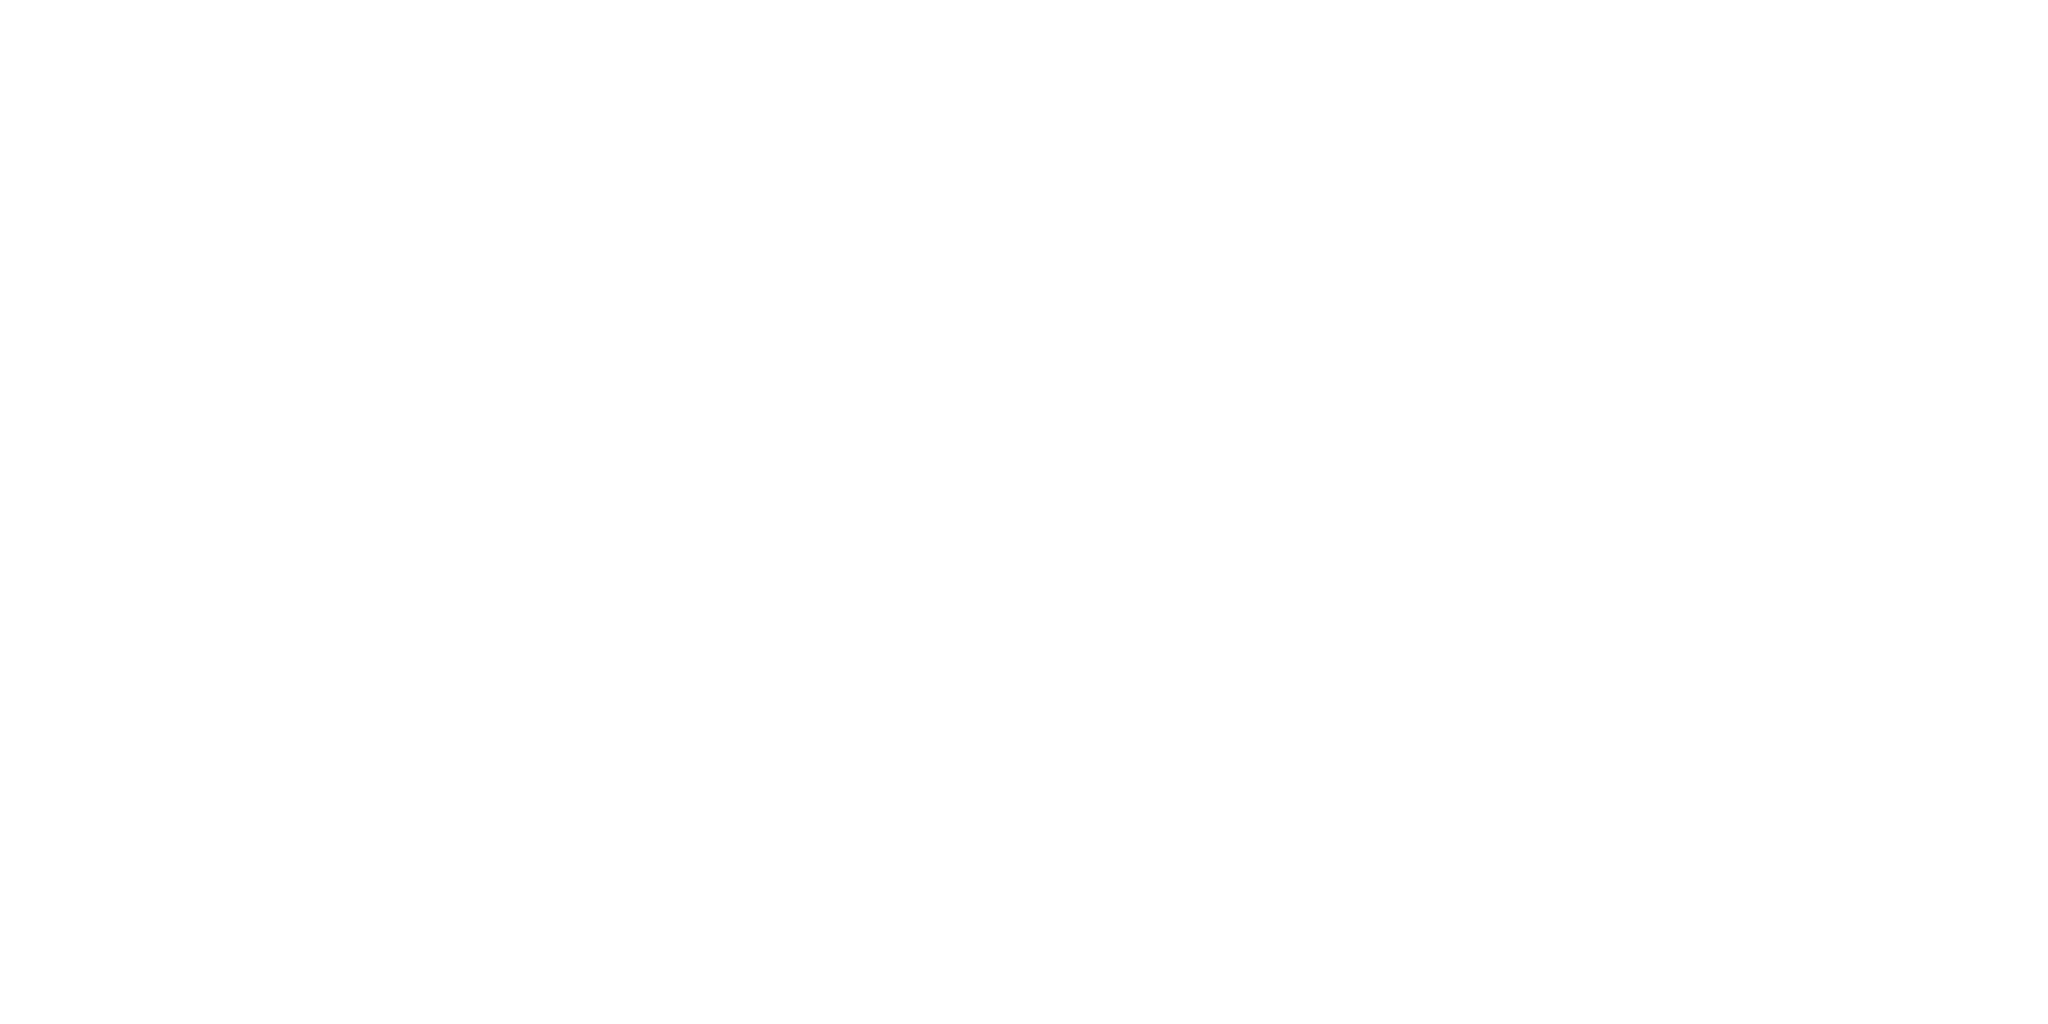
\includegraphics[width=\textwidth]{blank.png}}{flow.mp4}
    \caption{Samples from a normalising flow model created by OpenAI in 2018\footfullcite{Dhariwal_Kingma_2018}.}
\end{figure}
\end{frame}

\section{The CDF Method for One-Dimensional Codomains}

\begin{frame}[fragile]{The CDF Method}
Here we will look at one method for determining the CDF of the random variable \(Y = g\left(\bm{X}\right)\) for some function \(g: \mathcal{X}\rightarrow\mathcal{Y}\). We will constrain ourselves to dealing with cases where \(Y\) is one-dimensional.\onslide<2->{

\metroset{block=fill}\begin{alertblock}{The CDF Method}
Given \(Y = g\left(\bm{X}\right)\) and the CDF \(F_{\bm{X}}\) for \(\bm{X}\), we can find the CDF \(F_Y\) for \(Y\) with the following steps:
\begin{enumerate}[<+(1)->]
    \item Start by writing
    \begin{equation*}
        \begin{aligned}
            F_Y\left(y\right) &= \mathbb{P}\left(Y \leq y\right)\\
            &= \mathbb{P}\left(g\left(\bm{X}\right) \leq y\right)\,.
        \end{aligned}
    \end{equation*}
    \item Manipulate \(\mathbb{P}\left(g\left(\bm{X}\right) \leq y\right)\) until it is written in terms of known functions (e.g. \(F_{\bm{X}}\)). Substitute in these functions and simplify.
    \item (\textit{Optional}) Given the CDF, find the PMF/PDF.
\end{enumerate}
\end{alertblock}}
\end{frame}

\begin{frame}[fragile]{The CDF Method}
A reminder regarding step 3:
\begin{itemize}[<+->]
    \item For discrete \(Y\), we take differences of the CDF to find the PMF. E.g. \(f_Y\left(y\right) = F_Y\left(y\right) - F_Y\left(y - 1\right)\) for \(y\in\mathcal{Y}\) when the support is a subset of the integers. In general, \(\mathbb{P}\left(Y = y\right) = \mathbb{P}\left(Y \leq y\right) - \mathbb{P}\left(Y < y\right)\).
    \item For continuous \(Y\), we take the derivative of the CDF with respect to \(y\) to find the PDF: \(f_Y\left(y\right) = \diff{}{y}F_Y\left(y\right)\).
\end{itemize}
\end{frame}

\begin{frame}[fragile]{A Simple Discrete Example}
\metroset{block=fill}\begin{exampleblock}{Example 2}
Given \(X \sim \mathcal{U}\left\{1, 3\right\}\), what is the PMF of \(Y = 2X\)?\onslide<2->{

First, consider the supports. The support of \(X\) is \(\mathcal{X} = \left\{1, 2, 3\right\}\), so the support of \(Y\) will be \(\mathcal{Y} = \left\{2, 4, 6\right\}\). Also, we know that
\begin{equation*}
\begin{aligned}
    F_X\left(x\right) &= \begin{cases}
        0 & \textrm{if } x < 1\\
        \frac{1}{3} & \textrm{if } 1 \leq x < 2\\
        \frac{2}{3} & \textrm{if } 2 \leq x < 3\\
        1 & \textrm{if } x \geq 3
    \end{cases}\,,
\end{aligned}
\end{equation*}
so let's try to find an expression for \(F_Y\) in terms of \(F_X\).}
\end{exampleblock}
\end{frame}

\begin{frame}[fragile]{A Simple Discrete Example}
\metroset{block=fill}\begin{exampleblock}{Example 2}
The CDF for \(Y\) is given by
\begin{equation*}
\begin{aligned}
    F_Y\left(y\right) &= \mathbb{P}\left(Y \leq y\right)\\
    &= \mathbb{P}\left(2X \leq y\right)\\
    &= \mathbb{P}\left(X \leq \frac{y}{2}\right)\\
    &= F_X\left(\frac{y}{2}\right)\\
    &= \begin{cases}
        0 & \textrm{if } y < 2\\
        \frac{1}{3} & \textrm{if } 2 \leq y < 4\\
        \frac{2}{3} & \textrm{if } 4 \leq y < 6\\
        1 & \textrm{if } y \geq 6
    \end{cases}\,.
\end{aligned}
\end{equation*}
\end{exampleblock}
\end{frame}

\begin{frame}[fragile]{A Simple Discrete Example}
\metroset{block=fill}\begin{exampleblock}{Example 2}
For all \(y\in\mathcal{Y}\), the PMF is then given by
\begin{equation*}
\begin{aligned}
    f_Y\left(y\right) &= F_Y\left(y\right) - F_Y\left(y - 2\right)\\
    &= F_X\left(\frac{y}{2}\right) - F_X\left(\frac{y}{2} - 1\right)\\
    &= \begin{cases}
        \frac{1}{3} & \textrm{if } y\in\mathcal{Y}\\
        0 & \textrm{otherwise}
    \end{cases}\,.
\end{aligned}
\end{equation*}
\end{exampleblock}
\end{frame}

\begin{frame}[fragile]{A Simple Continuous Example}
\metroset{block=fill}\begin{exampleblock}{Example 3}
Given \(X \sim \mathcal{U}\left[0, 1\right]\), what is the PDF of \(Y = -2X\)?\onslide<2->{

First, consider the supports. The support of \(X\) is \(\mathcal{X} = \left[0, 1\right]\), so the support of \(Y\) will be \(\mathcal{Y} = \left[-2, 0\right]\). Also, we know that \(F_X\left(x\right) = x\) for \(x \in \mathcal{X}\), so let's try to find an expression for \(F_Y\) in terms of \(F_X\). The CDF for \(Y\) is given by
\begin{equation*}
\begin{aligned}
    F_Y\left(y\right) &= \mathbb{P}\left(Y \leq y\right)\\
    &= \mathbb{P}\left(-2X \leq y\right)\\
    &= \mathbb{P}\left(X \geq -\frac{y}{2}\right)\\
    &= 1 - \mathbb{P}\left(X \leq -\frac{y}{2}\right)\\
    &= 1 - F_X\left(-\frac{y}{2}\right)\\
    &= 1 + \frac{y}{2}\quad\textrm{for } y \in \mathcal{Y}\,.
\end{aligned}
\end{equation*}}
\end{exampleblock}
\end{frame}

\begin{frame}[fragile]{A Simple Continuous Example}
\metroset{block=fill}\begin{exampleblock}{Example 3}
For all \(y\in\mathcal{Y}\), the PDF is then given by
\begin{equation*}
\begin{aligned}
    f_Y\left(y\right) &= \diff{}{y}F_Y\left(y\right)\\
    &= \diff{}{y}\left(1 + \frac{y}{2}\right)\\
    &= \frac{1}{2}\,.
\end{aligned}
\end{equation*}
\end{exampleblock}\onslide<2->{

Take note that the support interval doubled in size, and the PDF halved in magnitude to compensate. This is in contrast to the discrete example, where the support size and probabilities remained the same.}
\end{frame}

\begin{frame}[fragile]{Non-Injective Examples}
So far our we have only considered injective functions in our examples. Let's consider some non-injective functions. These problems may require a bit more thought and effort.
\end{frame}

\begin{frame}[fragile]{Sums of Random Variables}
\metroset{block=fill}\begin{exampleblock}{Example 4}
Let \(X\) and \(Y\) be arbitrary independent random variables with supports \(\mathcal{X}\) and \(\mathcal{Y}\) respectively. What is the PMF/PDF of \(Z = X + Y\)?\onslide<2->{

Let's start with the CDF:
\begin{equation*}
\begin{aligned}
    F_Z\left(z\right) &= \mathbb{P}\left(Z \leq z\right)\\
    &= \mathbb{P}\left(X + Y \leq z\right)
\end{aligned}
\end{equation*}
\begin{columns}[t]
\begin{column}{0.425\textwidth}
Discrete \(X\):
\begin{equation*}
\begin{aligned}
    &= \sum_{x\in\mathcal{X}}\mathbb{P}\left(x + Y \leq z, X = x\right)\\
    &= \sum_{x\in\mathcal{X}}\mathbb{P}\left(Y \leq z - x\right)\mathbb{P}\left(X = x\right)\\
    &= \sum_{x\in\mathcal{X}}F_Y\left(z - x\right)f_X\left(x\right)
\end{aligned}
\end{equation*}
\end{column}
\begin{column}{0.425\textwidth}
Continuous \(X\):
\begin{equation*}
\begin{aligned}
    &= \int_{\mathcal{X}}\mathbb{P}\left(x + Y \leq z\right)f_X\left(x\right)\mathrm{d}x\\
    &= \int_{\mathcal{X}}\mathbb{P}\left(Y \leq z - x\right)f_X\left(x\right)\mathrm{d}x\\
    &= \int_{\mathcal{X}}F_Y\left(z - x\right)f_X\left(x\right)\mathrm{d}x
\end{aligned}
\end{equation*}
\end{column}
\end{columns}}
\end{exampleblock}
\end{frame}

\begin{frame}[fragile]{Sums of Random Variables}
\metroset{block=fill}\begin{exampleblock}{Example 4}
Now we can find the PMF/PDF. In the left column we assume the support of \(Y\) is a subset of the integers. In the right column we assume \(Y\) is continuous.
\begin{equation*}
    f_Z\left(z\right)
\end{equation*}
\begin{columns}[t]
\begin{column}{0.425\textwidth}
Discrete \(X\) and \(Y\):
\begin{equation*}
\begin{aligned}
    &= F_Z\left(z\right) - F_Z\left(z - 1\right)\\
    &= \sum_{x\in\mathcal{X}}\left(F_Y\left(z - x\right)\right.\\
    &\phantom{=}\quad \left.- F_Y\left(z - 1 - x\right)\right)f_X\left(x\right)\\
    &= \sum_{x\in\mathcal{X}}f_Y\left(z - x\right)f_X\left(x\right)
\end{aligned}
\end{equation*}
\end{column}
\begin{column}{0.425\textwidth}
Continuous \(X\) and \(Y\):
\begin{equation*}
\begin{aligned}
    &= \diff{}{z}F_Z\left(z\right)\\
    &= \int_{\mathcal{X}}\diff{}{z}F_Y\left(z - x\right)f_X\left(x\right)\mathrm{d}x\\
    &= \int_{\mathcal{X}}f_Y\left(z - x\right)f_X\left(x\right)\mathrm{d}x
\end{aligned}
\end{equation*}
\end{column}
\end{columns}

These operations are called convolutions.
\end{exampleblock}
\end{frame}

\begin{frame}[fragile]{Squaring a Gaussian}
\metroset{block=fill}\begin{exampleblock}{Example 5}
What is the PDF of \(Y = X^2\) given \(X\sim\mathcal{N}\left(0, 1\right)\)?\onslide<2->{

The CDF for \(Y\) is given by
\begin{equation*}
\begin{aligned}
    F_Y\left(y\right) &= \mathbb{P}\left(Y \leq y\right)\\
    &= \mathbb{P}\left(X^2 \leq y\right)\\
    &= \mathbb{P}\left(-\sqrt{y} \leq X \leq \sqrt{y}\right)\\
    &= \mathbb{P}\left(X \leq \sqrt{y}\right) - \mathbb{P}\left(X \leq -\sqrt{y}\right)\\
    &= F_X\left(\sqrt{y}\right) - F_X\left(-\sqrt{y}\right)\\
    &= \frac{1}{2}\left(1 + \href{https://en.wikipedia.org/wiki/Error_function}{\color{mLightBrown}{\mathrm{erf}}}\left(\sqrt{\frac{y}{2}}\right)\right) - \frac{1}{2}\left(1 + \mathrm{erf}\left(-\sqrt{\frac{y}{2}}\right)\right)\\
    &= \frac{1}{2}\left(\mathrm{erf}\left(\sqrt{\frac{y}{2}}\right) - \mathrm{erf}\left(-\sqrt{\frac{y}{2}}\right)\right)\,.
\end{aligned}
\end{equation*}}
\end{exampleblock}
\end{frame}

\begin{frame}[fragile]{Squaring a Gaussian}
\metroset{block=fill}\begin{exampleblock}{Example 5}
The PDF is then given by
\begin{equation*}
\begin{aligned}
    f_Y\left(y\right) &= \diff{}{y}F_Y\left(y\right)\\
    &= \diff{}{y}\frac{1}{2}\left(\mathrm{erf}\left(\sqrt{\frac{y}{2}}\right) - \mathrm{erf}\left(-\sqrt{\frac{y}{2}}\right)\right)\\
    &= \frac{1}{2}\left(\frac{2}{\sqrt{\pi}}e^{-\sfrac{y}{2}}\cdot\frac{1}{2}\sqrt{\frac{2}{y}}\cdot\frac{1}{2} + \frac{2}{\sqrt{\pi}}e^{-\sfrac{y}{2}}\cdot\frac{1}{2}\sqrt{\frac{2}{y}}\cdot\frac{1}{2}\right)\\
    &= \frac{1}{\sqrt{2\pi y}}e^{-\sfrac{y}{2}}\,.
\end{aligned}
\end{equation*}
\end{exampleblock}
\end{frame}

\begin{frame}[fragile]{The Maximum of a Set of Random Variables}
\metroset{block=fill}\begin{exampleblock}{Example 6}
If \(Y = \max\left\{X_1, \dots, X_n\right\}\) for \(n\) independent continuous random variables \(X_1, \dots, X_n\), what is the PDF of \(Y\)?\onslide<2->{

The CDF for \(Y\) is given by
\begin{equation*}
\begin{aligned}
    F_Y\left(y\right) &= \mathbb{P}\left(Y \leq y\right)\\
    &= \mathbb{P}\left(\max\left\{X_1, \dots, X_n\right\} \leq y\right)\\
    &= \mathbb{P}\left(X_1 \leq y, \dots, X_n \leq y\right)\\
    &= \prod_{i=1}^n\mathbb{P}\left(X_i \leq y\right)\\
    &= \prod_{i=1}^n F_{X_i}\left(y\right)\,.
\end{aligned}
\end{equation*}}
\end{exampleblock}
\end{frame}

\begin{frame}[fragile]{The Maximum of a Set of Random Variables}
\metroset{block=fill}\begin{exampleblock}{Example 6}
The PDF for \(Y\) is then given by
\begin{equation*}
\begin{aligned}
    f_Y\left(y\right) &= \diff{}{y}F_Y\left(y\right)\\
    &= \diff{}{y}\prod_{i=1}^n F_{X_i}\left(y\right)\\
    &= \sum_{i=1}^n f_{X_i}\left(y\right)\prod_{j\neq i} F_{X_j}\left(y\right)\,.
\end{aligned}
\end{equation*}
\end{exampleblock}
\end{frame}

\begin{frame}[standout]
Intermission
\end{frame}

\section{The Method of Transformations for Bijective Functions}

\begin{frame}[fragile]{Bijective Functions of Discrete Random Variables}
If \(\bm{g}\) is a bijective function and \(\bm{X}\) is a discrete random variable with PMF \(f_{\bm{X}}\), then \(\bm{Y} = \bm{g}\left(\bm{X}\right)\) has PMF \(f_{\bm{Y}}\left(\bm{y}\right) = f_{\bm{X}}\left(\bm{g}^{-1}\left(\bm{y}\right)\right)\). I.e. the mapping may change the support, but doesn't change probabilities. Because the probabilities don't change, \(f_{\bm{Y}}\left(\bm{y}\right)\) still sums to one over the transformed support.\onslide<2->{

\textit{Proof}:

\begin{equation*}
\begin{aligned}
    \mathbb{P}\left(\bm{Y} = \bm{y}\right) &= \mathbb{P}\left(\bm{g}\left(\bm{X}\right) = \bm{y}\right)\\
    f_{\bm{Y}}\left(\bm{y}\right) &= \mathbb{P}\left(\bm{X} = \bm{g}^{-1}\left(\bm{y}\right)\right)\\
    &= f_{\bm{X}}\left(\bm{g}^{-1}\left(\bm{y}\right)\right)
\end{aligned}
\end{equation*}
\qed

The first example in this lecture demonstrates this well.}
\end{frame}

\begin{frame}[fragile]{Bijective Functions of Continuous Random Variables}
The discrete case is very simple. The continuous case is more complicated.
\metroset{block=fill}\begin{alertblock}{The Method of Transformations}
For continuous random variables \(\bm{X}\) and \(\bm{Y} = \bm{g}\left(\bm{X}\right)\), where \(\bm{g}\) is a bijective function, we have the following relationship between the PDFs \(f_{\bm{X}}\) and \(f_{\bm{Y}}\):
\begin{equation*}
    \begin{aligned}
        f_{\bm{Y}}\left(\bm{y}\right) &= f_{\bm{X}}\left(\bm{g}^{-1}\left(\bm{y}\right)\right)\left|\det\left(\mathrm{D}\bm{g}^{-1}\left(\bm{y}\right)\right)\right|\\
        &= f_{\bm{X}}\left(\bm{g}^{-1}\left(\bm{y}\right)\right)\left|\det\left(\mathrm{D}\bm{g}\left(\bm{g}^{-1}\left(\bm{y}\right)\right)\right)\right|^{-1}\,.
    \end{aligned}
\end{equation*}
The notation \(\mathrm{D}\bm{g}\left(\bm{x}\right)\) means "the Jacobian of \(\bm{g}\), evaluated at \(\bm{x}\)".
\end{alertblock}\onslide<2->{

In the one-dimensional case, this simplifies to:
\begin{equation*}
    \begin{aligned}
        f_{Y}\left(y\right) &= f_{X}\left(g^{-1}\left(y\right)\right)\left|\diff{g^{-1}}{y}\left(y\right)\right|\\
        &= f_{X}\left(g^{-1}\left(y\right)\right)\left|\diff{g}{x}\left(g^{-1}\left(y\right)\right)\right|^{-1}\,.
    \end{aligned}
\end{equation*}}
\end{frame}

\begin{frame}[fragile]{Bijective Functions of Continuous Random Variables}
\textit{Proof}:

Let \(A\) be some subset of the support of \(\bm{Y}\). Then
\begin{equation*}
    \begin{aligned}
        \mathbb{P}\left(\bm{Y} \in A\right) &= \mathbb{P}\left(\bm{g}\left(\bm{X}\right) \in A\right)\\
        \int_A f_{\bm{Y}}\left(\bm{y}\right)\mathrm{d}\bm{y} &= \mathbb{P}\left(\bm{X} \in \bm{g}^{-1}\left(A\right)\right)\\
        &= \int_{\bm{g}^{-1}\left(A\right)} f_{\bm{X}}\left(\bm{x}\right)\mathrm{d}\bm{x}\,.
    \end{aligned}
\end{equation*}
Performing integration by substitution on the right side of the equation with \(\bm{y} = \bm{g}\left(\bm{x}\right)\), giving us \(\mathrm{d}\bm{x} = \left|\det\left(\mathrm{D}\bm{g}^{-1}\left(\bm{y}\right)\right)\right|\mathrm{d}\bm{y}\), we see that
\begin{equation*}
    \begin{aligned}
        \int_A f_{\bm{Y}}\left(\bm{y}\right)\mathrm{d}\bm{y} &= \int_{A} f_{\bm{X}}\left(\bm{g}^{-1}\left(\bm{y}\right)\right)\left|\det\left(\mathrm{D}\bm{g}^{-1}\left(\bm{y}\right)\right)\right|\mathrm{d}\bm{y}\\
        \therefore f_{\bm{Y}}\left(\bm{y}\right) &= f_{\bm{X}}\left(\bm{g}^{-1}\left(\bm{y}\right)\right)\left|\det\left(\mathrm{D}\bm{g}^{-1}\left(\bm{y}\right)\right)\right|\,.
    \end{aligned}
\end{equation*}\onslide<2->{
Alternatively, we could have used \(\mathrm{d}\bm{y} = \left|\det\left(\mathrm{D}\bm{g}\left(\bm{x}\right)\right)\right|\mathrm{d}\bm{x}\) in the substitution. Remember, the Jacobian of a function is the same as the reciprocal of the Jacobian of the inverse function.}
\qed
\end{frame}

\begin{frame}[fragile]{The Log-Normal Distribution}
\metroset{block=fill}\begin{exampleblock}{Example 7}
If \(Y = e^X\) and \(X\sim\mathcal{N}\left(\mu,\sigma^2\right)\), then \(Y\) is log-normally distributed. What is the PDF of the log-normal distribution?\onslide<2->{

The support and PDF of \(X\) are \(\left(-\infty,\infty\right)\) and
\begin{equation*}
    f_X\left(x\right) = \frac{1}{\sqrt{2\pi\sigma^2}}\exp\left(-\frac{\left(x - \mu\right)^2}{2\sigma^2}\right)
\end{equation*}
respectively. Clearly the support of \(Y\) will be \(\left[0, \infty\right)\).}
\end{exampleblock}
\end{frame}

\begin{frame}[fragile]{The Log-Normal Distribution}
\metroset{block=fill}\begin{exampleblock}{Example 7}
Writing \(x = \log\left(y\right)\), we see that \(\frac{\mathrm{d}x}{\mathrm{d}y} = \frac{1}{y}\). Given this information we proceed as follows:
\begin{equation*}
    \begin{aligned}
        f_{Y}\left(y\right) &= f_{X}\left(x\right)\left|\diff{x}{y}\right|\\
        &= f_{X}\left(\log\left(y\right)\right)\left|\frac{1}{y}\right|\\
        &= \frac{1}{y\sqrt{2\pi\sigma^2}}\exp\left(-\frac{\left(\log\left(y\right) - \mu\right)^2}{2\sigma^2}\right)\,.
    \end{aligned}
\end{equation*}
\end{exampleblock}
\end{frame}

\begin{frame}[fragile]{Inverse Transform Sampling}
\metroset{block=fill}\begin{exampleblock}{Example 8}
The PDF of a univariate distribution with support \(\mathcal{Y}\) is known, but we need a way to sample from it. Given a sample \(x\) from \(\mathcal{U}\left[0, 1\right]\), what must the bijective and strictly increasing function \(g: \left[0,1\right]\rightarrow\mathcal{Y}\) be such that \(g\left(x\right)\) is a sample from the desired distribution?\onslide<2->{

Let \(Y = g\left(X\right)\) for \(X\sim\mathcal{U}\left[0, 1\right]\). \(f_{X}\left(x\right) = 1\) on the support. As \(g\) is strictly increasing, \(\frac{\mathrm{d}g}{\mathrm{d}x} > 0\), which also means \(\frac{\mathrm{d}g^{-1}}{\mathrm{d}y} > 0\). Then
\begin{equation*}
    \begin{aligned}
        f_{Y}\left(y\right) &= f_{X}\left(g^{-1}\left(y\right)\right)\left|\diff{g^{-1}}{y}\left(y\right)\right|\\
        &= \diff{g^{-1}}{y}\left(y\right)\\
        g^{-1}\left(y\right) &= \int_{-\infty}^y f_{Y}\left(z\right)\mathrm{d}z + c\\
        &= F_{Y}\left(y\right) + c\,.
    \end{aligned}
\end{equation*}}
\end{exampleblock}
\end{frame}

\begin{frame}[fragile]{Inverse Transform Sampling}
\metroset{block=fill}\begin{exampleblock}{Example 8}
When \(y\rightarrow-\infty\) we have:
\begin{equation*}
    \begin{aligned}
        \lim_{y\rightarrow-\infty}g^{-1}\left(y\right) &= \lim_{y\rightarrow-\infty}F_{Y}\left(y\right) + c\\
        0 &= 0 + c\\
        c &= 0\,.
    \end{aligned}
\end{equation*}
Therefore, \(g\left(x\right) = F_{Y}^{-1}\left(x\right)\).
\end{exampleblock}\onslide<2->{
We have seen a proof for the inverse transform sampling method in a previous lecture. This is an alternative proof for why this method works.}
\end{frame}

\begin{frame}[fragile]{Linear Transformations of Multivariate Gaussians}
\metroset{block=fill}\begin{exampleblock}{Example 9}
Given \(\bm{X}\sim\mathcal{N}\left(\bm{0}, I\right)\) with support \(\mathbb{R}^n\), what is the PDF of \(\bm{Y} = A\bm{X}\) for some real and invertible \(n\times n\) matrix \(A\)?\onslide<2->{

We have \(f_{\bm{X}}\left(\bm{x}\right) = \left(2\pi\right)^{-\sfrac{n}{2}}\exp\left(-\frac{1}{2}\bm{x}^T\bm{x}\right)\). Let's start by recognising that \(\bm{x} = A^{-1}\bm{y}\) and \(\mathrm{D}\bm{y}\left(\bm{x}\right) = A\). Given this information we proceed as follows:
\begin{equation*}
    \begin{aligned}
        f_{\bm{Y}}\left(\bm{y}\right) &= f_{\bm{X}}\left(\bm{x}\right)\left|\det\left(\mathrm{D}\bm{y}\left(\bm{x}\right)\right)\right|^{-1}\\
        &= f_{\bm{X}}\left(A^{-1}\bm{y}\right)\left|\det\left(A\right)\right|^{-1}\\
        &= \left(2\pi\right)^{-\sfrac{n}{2}}\exp\left(-\frac{1}{2}\left(A^{-1}\bm{y}\right)^T\left(A^{-1}\bm{y}\right)\right)\left(\det\left(A\right)\det\left(A\right)\right)^{-\sfrac{1}{2}}\\
        &= \left(2\pi\right)^{-\sfrac{n}{2}}\exp\left(-\frac{1}{2}\bm{y}^T\left(A^T\right)^{-1}A^{-1}\bm{y}\right)\left(\det\left(A\right)\det\left(A^T\right)\right)^{-\sfrac{1}{2}}\\
        &= \left(2\pi\right)^{-\sfrac{n}{2}}\left(\det\left(AA^T\right)\right)^{-\sfrac{1}{2}}\exp\left(-\frac{1}{2}\bm{y}^T\left(AA^T\right)^{-1}\bm{y}\right)\,.
    \end{aligned}
\end{equation*}
Therefore \(\bm{Y}\) is also multivariate Gaussian. \(Y\sim\mathcal{N}\left(\bm{0}, AA^T\right)\).}
\end{exampleblock}
\end{frame}

\begin{frame}[standout]
Intermission
\end{frame}

\section{The Method of Transformations for Non-Injective, Surjective Functions}

\begin{frame}[fragile]{From Non-Injectivity to Bijectivity}
The method of transformations is only applicable in the case of bijective functions. There is no standard way of dealing with all non-bijective functions, but here we will discuss a helpful method for dealing with some non-injective, surjective functions.\onslide<2->{

\metroset{block=fill}\begin{alertblock}{The Method of Transformations for Non-Injective, Surjective Functions}
For continuous random variables \(\bm{X}_1\) and \(\bm{Y}_1 = \bm{g}\left(\bm{X}_1\right)\), where \(\bm{g}\) is a non-injective, surjective function, we can attempt to find the PDF \(f_{\bm{Y}_1}\) for \(\bm{Y}_1\) with the following steps:
\begin{enumerate}[<+(1)->]
    \item Introduce new random variables \(\bm{X}_2\) and \(\bm{Y}_2\) as needed, in addition to \(\bm{X}_1\) and \(\bm{Y}_1\). Create a new bijective function \(\left(\bm{Y}_1, \bm{Y}_2\right) = \bm{h}\left(\bm{X}_1, \bm{X}_2\right)\) which keeps the marginal distribution of \(\bm{Y}_1\) unchanged.
    \item Apply the method of transformations on the bijective problem.
    \item Find the marginal distribution of \(\bm{Y}_1\) by marginalising out \(\bm{Y}_2\).
\end{enumerate}
\end{alertblock}}
\end{frame}

\begin{frame}[fragile]{Sums of Independent Continuous Random Variables}
\metroset{block=fill}\begin{exampleblock}{Example 10}
Let \(X_1\) and \(X_2\) be independent continuous random variables with supports \(\mathcal{X}_1\) and \(\mathcal{X}_2\) respectively. What is the distribution of \(Y_1 = X_1 + X_2\)?\onslide<2->{

This function is non-injective. Let's make a bijective one to help us solve the problem. In addition to \(Y_1 = X_1 + X_2\), let's introduce \(Y_2 = X_2\). Given \(Y_1\) and \(Y_2\), we can recover \(X_1\) and \(X_2\), so this mapping is bijective.

Writing this function in the form \(\bm{h}\left(\bm{x}\right) = \left(x_1 + x_2, x_2\right)\) and letting \(\bm{y} = \bm{h}\left(\bm{x}\right)\), we see the Jacobian is
\begin{equation*}
    \mathrm{D}\bm{h}\left(\bm{x}\right) = \begin{pmatrix}
        1 & 1\\0 & 1
    \end{pmatrix}\,.
\end{equation*}}
\end{exampleblock}
\end{frame}

\begin{frame}[fragile]{Sums of Independent Continuous Random Variables}
\metroset{block=fill}\begin{exampleblock}{Example 10}
Now, applying the method of transformations:
\begin{equation*}
    \begin{aligned}
        f_{\bm{Y}}\left(\bm{y}\right) &= f_{\bm{X}}\left(\bm{x}\right)\left|\det\left(\mathrm{D}\bm{h}\left(\bm{x}\right)\right)\right|^{-1}\\
        &= f_{\bm{X}}\left(y_1 - y_2, y_2\right)\left|\det\begin{pmatrix}
            1 & 1\\
            0 & 1
        \end{pmatrix}\right|^{-1}\\
        &= f_{\bm{X}}\left(y_1 - y_2, y_2\right)\,.
    \end{aligned}
\end{equation*}
\end{exampleblock}
\end{frame}

\begin{frame}[fragile]{Sums of Independent Continuous Random Variables}
\metroset{block=fill}\begin{exampleblock}{Example 10}
Now we just need to find the marginal distribution of \(Y_1\). To do this, recognise that the support of \(Y_2\) is identical to \(X_2\).
\begin{equation*}
    \begin{aligned}
        f_{Y_1}\left(y_1\right) &= \int_{\mathcal{Y}_2}f_{\bm{Y}}\left(\bm{y}\right)\mathrm{d}y_2\\
        &= \int_{\mathcal{Y}_2}f_{\bm{X}}\left(y_1 - y_2, y_2\right)\mathrm{d}y_2\\
        &= \int_{\mathcal{Y}_2}f_{X_1}\left(y_1 - y_2\right)f_{X_2}\left(y_2\right)\mathrm{d}y_2\\
        &= \int_{\mathcal{X}_2}f_{X_1}\left(y_1 - x_2\right)f_{X_2}\left(x_2\right)\mathrm{d}x_2\,.
    \end{aligned}
\end{equation*}
This convolution agrees with the result we got earlier in the lecture using the CDF method.
\end{exampleblock}
\end{frame}

\begin{frame}[fragile]{The Sum of Gaussian Random Variables is Gaussian}
We can prove that the sum of independent univariate Gaussian random variables is also Gaussian using convolutions, but this proof involves a particularly horrible mess of algebra. \href{https://en.wikipedia.org/wiki/Sum_of_normally_distributed_random_variables#Proof_using_convolutions}{\color{mLightBrown}{Here's the proof}} for anyone wanting to suffer.\onslide<2->{

To summarise, if \(X\sim\mathcal{N}\left(\mu_X,\sigma_X^2\right)\) and \(Y\sim\mathcal{N}\left(\mu_Y,\sigma_Y^2\right)\), then
\begin{equation*}
X + Y\sim\mathcal{N}\left(\mu_X + \mu_Y,\sigma_X^2 + \sigma_Y^2\right)\,.
\end{equation*}}\onslide<3>{
This is also true for independent multivariate Gaussian random variables. If \(\bm{X}\sim\mathcal{N}\left(\bm{\mu}_{\bm{X}},\Sigma_{\bm{X}}\right)\) and \(\bm{Y}\sim\mathcal{N}\left(\bm{\mu}_{\bm{Y}},\Sigma_{\bm{Y}}\right)\), then
\begin{equation*}
    \bm{X}+\bm{Y}\sim\mathcal{N}\left(\bm{\mu}_{\bm{X}} + \bm{\mu}_{\bm{Y}},\Sigma_{\bm{X}} + \Sigma_{\bm{Y}}\right)\,.
\end{equation*}}
\end{frame}

\begin{frame}[fragile]{The Dirac Delta}
Before continuing, we need to introduce the Dirac delta "function". It isn't really a regular function, but you can just consider it one for now. It is very loosely defined as
\begin{equation*}
    \delta\left(x\right) \simeq
    \begin{cases}
        \infty & \textrm{if } x = 0\\
        0 & \textrm{otherwise}
    \end{cases}\,,
\end{equation*}
and has the following important properties:
\begin{itemize}[<+->]
    \item Can be used as a PDF:
    \begin{equation*}
        \int_{-\infty}^\infty\delta\left(x\right)\mathrm{d}x = 1\,.
    \end{equation*}
    \item Is easy to integrate:
    \begin{equation*}
        \int_{-\infty}^\infty g\left(x\right)\delta\left(x - a\right)\mathrm{d}x = g\left(a\right)\,.
    \end{equation*}
\end{itemize}
\end{frame}

\begin{frame}[fragile]{The Dirac Delta}
The Dirac delta defines a deterministic distribution, where a single outcome occurs with probability 1. You can consider it as a normal distribution with mean 0 in the limit of the standard deviation approaching 0:
\begin{equation*}
    \delta\left(x\right) = \lim_{\sigma\rightarrow 0^+}\frac{1}{\sqrt{2\pi\sigma^2}}e^{-\frac{x^2}{2\sigma^2}}\,.
\end{equation*}\onslide<2->{
One more useful relationship is as follows. If a function \(g\) has \(n\) real roots/zeros \(x_1, \dots, x_n\), then
\begin{equation*}
    \delta\left(g\left(x\right)\right) = \sum_{i = 1}^n \frac{\delta\left(x - x_i\right)}{\left|g'\left(x_i\right)\right|}\,.
\end{equation*}

We will now see an example of how to use a Dirac delta.}
\end{frame}

\begin{frame}[fragile]{Squaring a Gaussian}
\metroset{block=fill}\begin{exampleblock}{Example 11}
What is the PDF of \(Y_1 = g\left(X_1\right)\) given \(X_1\sim\mathcal{N}\left(0, 1\right)\), \(g: \mathbb{R} \setminus \left\{0\right\}\rightarrow\left(0,\infty\right)\), and \(g\left(x\right) = x^2\)? Let's use the method of transformations.\onslide<2->{

\(g\) is surjective, but not injective. Let's address this by introducing a new function \(\bm{h}:\mathbb{R}^2 \setminus \left\{\left(0,0\right)\right\}\rightarrow\mathbb{R}^2 \setminus \left\{\left(0,0\right)\right\}\) defined by
\begin{equation*}
    \bm{h}\left(\bm{x}\right) = \left(x_1x_2, x_2\right)\,.
\end{equation*}
This is a bijective function, with \(\bm{y} = \bm{h}\left(\bm{x}\right)\) having the inverse
\begin{equation*}
    \bm{h}^{-1}\left(\bm{y}\right) = \left(\frac{y_1}{y_2}, y_2\right)\,.
\end{equation*}
Our plan here is to force \(x_1\) and \(x_2\) to take the same value, thus resulting in \(y_1 = x_1^2\).}
\end{exampleblock}
\end{frame}

\begin{frame}[fragile]{Squaring a Gaussian}
\metroset{block=fill}\begin{exampleblock}{Example 11}
Now that we've defined a bijective function, let's consider the random vector \(\bm{Y} = \bm{h}\left(\bm{X}\right)\) with \(X_1\sim\mathcal{N}\left(0, 1\right)\) and the distribution of \(X_2\mid X_1\) being deterministic. Specifically, the conditional PDF for \(X_2\mid X_1\) should be \(\delta\left(x_2 - x_1\right)\). Now, applying the method of transformations:
\begin{equation*}
    \begin{aligned}
        f_{\bm{Y}}\left(\bm{y}\right) &= f_{\bm{X}}\left(\bm{h}^{-1}\left(\bm{y}\right)\right)\left|\det\left(\mathrm{D}\bm{h}^{-1}\left(\bm{y}\right)\right)\right|\\
        &= f_{\bm{X}}\left(\frac{y_1}{y_2}, y_2\right)\left|\det\begin{pmatrix}
            \frac{1}{y_2} & -\frac{y_1}{y_2^2}\\
            0 & 1
        \end{pmatrix}\right|\\
        &= f_{\bm{X}}\left(\frac{y_1}{y_2}, y_2\right)\left|\frac{1}{y_2}\right|\\
        &= f_{X_1}\left(\frac{y_1}{y_2}\right)f_{X_2\mid X_1}\left(y_2\;\middle|\;\frac{y_1}{y_2}\right)\left|\frac{1}{y_2}\right|\\
        &= f_{X_1}\left(\frac{y_1}{y_2}\right)\delta\left(y_2 - \frac{y_1}{y_2}\right)\left|\frac{1}{y_2}\right|\,.
    \end{aligned}
\end{equation*}
\end{exampleblock}
\end{frame}

\begin{frame}[fragile]{Squaring a Gaussian}
\metroset{block=fill}\begin{exampleblock}{Example 11}
We have the joint distribution of \(Y_1\) and \(Y_2\). Let's find the marginal of \(Y_1\). First we need to decompose the Dirac delta. The roots of \(y_2 - \frac{y_1}{y_2}\) are \(y_2 = \pm \sqrt{y_1}\). The derivative of \(y_2 - \frac{y_1}{y_2}\) is \(1 + \frac{y_1}{y_2^2}\) which evaluates to 2 at the roots. Now we can continue:
\begin{equation*}
    \begin{aligned}
        f_{Y_1}\left(y_1\right) &= \int_{\mathbb{R}}f_{\bm{Y}}\left(\bm{y}\right)\mathrm{d}y_2\\
        &= \int_{\mathbb{R}}f_{X_1}\left(\frac{y_1}{y_2}\right)\delta\left(y_2 - \frac{y_1}{y_2}\right)\left|\frac{1}{y_2}\right|\mathrm{d}y_2\\
        &= \int_{\mathbb{R}}f_{X_1}\left(\frac{y_1}{y_2}\right)\cdot\frac{1}{2}\left(\delta\left(y_2 + \sqrt{y_1}\right) + \delta\left(y_2 - \sqrt{y_1}\right)\right)\left|\frac{1}{y_2}\right|\mathrm{d}y_2\\
        &= \frac{1}{2}\int_{\mathbb{R}}f_{X_1}\left(\frac{y_1}{y_2}\right)\delta\left(y_2 + \sqrt{y_1}\right)\left|\frac{1}{y_2}\right|\mathrm{d}y_2\\
        &\phantom{=}\quad + \frac{1}{2}\int_{\mathbb{R}}f_{X_1}\left(\frac{y_1}{y_2}\right)\delta\left(y_2 - \sqrt{y_1}\right)\left|\frac{1}{y_2}\right|\mathrm{d}y_2
    \end{aligned}
\end{equation*}
\end{exampleblock}
\end{frame}

\begin{frame}[fragile]{Squaring a Gaussian}
\metroset{block=fill}\begin{exampleblock}{Example 11}
\begin{equation*}
    \begin{aligned}
        &= \frac{1}{2}f_{X_1}\left(-\sqrt{y_1}\right)\left|\frac{-1}{\sqrt{y_1}}\right| + \frac{1}{2}f_{X_1}\left(\sqrt{y_1}\right)\left|\frac{1}{\sqrt{y_1}}\right|\\
        &= \frac{1}{2\sqrt{y_1}}\left(\frac{1}{\sqrt{2\pi}}\exp\left(-\frac{\left(-\sqrt{y_1}\right)^2}{2}\right) + \frac{1}{\sqrt{2\pi}}\exp\left(-\frac{\left(\sqrt{y_1}\right)^2}{2}\right)\right)\\
        &= \frac{1}{\sqrt{2\pi y_1}}\exp\left(-\frac{y_1}{2}\right)\,.
    \end{aligned}
\end{equation*}
\end{exampleblock}

This agrees with the result we got using the CDF method earlier. By the way, this is a chi-squared distribution.
\end{frame}

\begin{frame}[fragile]{Another Resource}
For a more comprehensive overview of the tools available to deal with functions of continuous random variables, take a look at this \href{https://en.wikibooks.org/wiki/Probability/Transformation_of_Probability_Densities}{\color{mLightBrown}{Wikibook}}.
\end{frame}

\section{Dynamical Systems as Functions: A Fun Proof to Look at After the Course}

\begin{frame}[fragile]{Tying Together the Modules in the Program}
This is a bonus section. It covers concepts from linear algebra, calculus, probability, and differential equations, but I don't expect anyone to grasp it immediately even after covering these modules. Treat it as a challenge \emoji{smirk}.

Here we will use \(\bm{x}_t\) as shorthand for \(\bm{x}\left(t\right)\).

Say we have some stochastic process \(\left\{\bm{X}_t \;\middle|\; t \in \left[0,\infty\right)\right\}\). We know the PDF of \(\bm{X}_0\) as well as the ODE that determines \(\bm{X}_t\) at all times \(t > 0\). If we have \(\bm{X}_0 \sim f_0\) and ODE
\begin{equation*}
    \diff{\bm{X}_t}{t} = \bm{g}\left(\bm{X}_t\right),
\end{equation*}
then what is the PDF \(f_t\) of \(\bm{X}_t\)?
\end{frame}

\begin{frame}[fragile]{Prerequisite: Flow Functions}
If we have an ODE, an initial state \(\bm{x}_s\), and a length of time \(t\) to run the dynamics for, then \(\bm{x}_{s + t}\) is determined by a function of \(\bm{x}_s\) and \(t\). If
\begin{equation*}
    \diff{\bm{x}_t}{t} = \bm{g}\left(\bm{x}_t\right),
\end{equation*}
 then we define this function \(\bm{\varphi}: \mathcal{X}\times\mathbb{R} \rightarrow \mathcal{X}\) as
 \begin{equation*}
 \begin{aligned}
     \bm{\varphi}\left(\bm{x}_s, t\right) &= \bm{x}_s + \int_s^{s+t} \bm{g}\left(\bm{x}_\tau\right) \mathrm{d}\tau\\
     &= \bm{x}_{s+t}
 \end{aligned}
 \end{equation*}
 This function is called a flow, and is often written as \(\bm{\varphi}^t\left(\bm{x_s}\right)\). Take note that \(\bm{\varphi}^s \circ \bm{\varphi}^t = \bm{\varphi}^{s+t}\).
\end{frame}

\begin{frame}[fragile]{How the PDF Warps Over Time}
Back to our original question: what is the PDF \(f_t\) of \(\bm{X}_t\)? It is given by
\begin{equation*}
    f_t\left(\bm{x}_t\right) = f_0\left(\bm{\varphi}^{-t}\left(\bm{x}_t\right)\right)\exp\left(\int_t^0 \nabla\cdot\bm{g}\left(\bm{x}_\tau\right)\mathrm{d}\tau\right)\,.
\end{equation*}

\textit{Proof}:

We need to find the change in volume over the trajectory taken by the dynamics. Here \(D\bm{\varphi}^t\) is the Jacobian of the flow \(\bm{\varphi}\) of the dynamics at time \(t\). Let's start with \href{https://en.wikipedia.org/wiki/Jacobi\%27s_formula}{\color{mLightBrown}{Jacobi's formula}}:
\begin{equation*}\begin{aligned}
    \diff{}{t}\det\left(D\bm{\varphi}^t\left(\bm{x}_0\right)\right) &= \det\left(D\bm{\varphi}^t\left(\bm{x}_0\right)\right) \tr\left(D\bm{\varphi}^t\left(\bm{x}_0\right)^{-1} \diff{}{t}D\bm{\varphi}^t\left(\bm{x}_0\right)\right)\,.
\end{aligned}\end{equation*}
\end{frame}

\begin{frame}[fragile]{How the PDF Warps Over Time}
Therefore, considering the derivative of logarithms:
\begin{equation*}\begin{aligned}
    \diff{}{t}\log\left(\det\left(D\bm{\varphi}^t\left(\bm{x}_0\right)\right)\right) &= \tr\left(D\bm{\varphi}^t\left(\bm{x}_0\right)^{-1} \diff{}{t}D\bm{\varphi}^t\left(\bm{x}_0\right)\right)\\
    &= \tr\left(D\bm{\varphi}^{-t}\left(\bm{\varphi}^t\left(\bm{x}_0\right)\right) D\diff{\bm{\varphi}^t}{t}\left(\bm{x}_0\right)\right)\\
    &= \tr\left(D\bm{\varphi}^{-t}\left(\bm{\varphi}^t\left(\bm{x}_0\right)\right) D\left(\bm{g}\circ\bm{\varphi}^t\right)\left(\bm{x}_0\right)\right)\\
    &= \tr\left(D\left(\bm{g}\circ\bm{\varphi}^t\circ\bm{\varphi}^{-t}\right)\left(\bm{\varphi}^t\left(\bm{x}_0\right)\right)\right)\\
    &= \tr\left(D\bm{g}\left(\bm{x}_t\right)\right)\\
    &= \nabla\cdot \bm{g}\left(\bm{x}_t\right)\,.
\end{aligned}\end{equation*}
\end{frame}

\begin{frame}[fragile]{How the PDF Warps Over Time}
Hence, the log Jacobian determinant of the flow over time \(t\) is given by
\begin{equation*}\begin{aligned}
    \log\left(\det\left(D\bm{\varphi}^t\left(\bm{x}_0\right)\right)\right) &= \log\left(\det\left(D\bm{\varphi}^0\left(\bm{x}_0\right)\right)\right) + \int_0^t \nabla\cdot\bm{g}\left(\bm{x}_\tau\right)\mathrm{d}\tau\\
    &= \log\left(\det\left(I\right)\right) + \int_0^t \nabla\cdot\bm{g}\left(\bm{x}_\tau\right)\mathrm{d}\tau\\
    &= \int_0^t \nabla\cdot\bm{g}\left(\bm{x}_\tau\right)\mathrm{d}\tau\,.
\end{aligned}\end{equation*}
Starting with \(\bm{x}_t\) and integrating backwards in time, we get
\begin{equation*}\begin{aligned}
    \log\left(\det\left(D\bm{\varphi}^t\left(\bm{\varphi}^{-t}\left(\bm{x}_t\right)\right)\right)\right) &= -\int_t^0 \nabla\cdot\bm{g}\left(\bm{x}_\tau\right)\mathrm{d}\tau\\
    \det\left(D\bm{\varphi}^t\left(\bm{\varphi}^{-t}\left(\bm{x}_t\right)\right)\right) &= \exp\left(-\int_t^0 \nabla\cdot\bm{g}\left(\bm{x}_\tau\right)\mathrm{d}\tau\right)\,.
\end{aligned}\end{equation*}
\end{frame}

\begin{frame}[fragile]{How the PDF Warps Over Time}
Finally, using the method of transformations, we have
\begin{equation*}
    \begin{aligned}
        f_t\left(\bm{x}_t\right) &= f_0\left(\bm{\varphi}^{-t}\left(\bm{x}_t\right)\right)\left|\det\left(D\bm{\varphi}^t\left(\bm{\varphi}^{-t}\left(\bm{x}_t\right)\right)\right)\right|^{-1}\\&= f_0\left(\bm{\varphi}^{-t}\left(\bm{x}_t\right)\right)\exp\left(\int_t^0 \nabla\cdot\bm{g}\left(\bm{x}_\tau\right)\mathrm{d}\tau\right)\,.
    \end{aligned}
\end{equation*}
\qed

If we can sample from \(f_0\) and approximately simulate the given dynamics, we can get approximate samples from \(f_t\) for any length of time \(t\). Of equal importance, we can also approximately calculate \(f_t\left(\bm{x}_t\right)\) using the formula above. Notice how \(f_t\) starts at \(f_0\) and smoothly warps over time.
\end{frame}

\begin{frame}[standout]
The End
\end{frame}

\end{document}